\chapter{Introduction}
\label{chap:introduction}


% Einträge im Verzeichnis erscheinen lassen ohne hier eine Referenz einzufügen
\nocite{kopka:band1}
\nocite{raichle:bibtex_programmierung}
\nocite{MiKTeX}
\nocite{KOMA}
\nocite{TeXnicCenter}
\nocite{Marti06}
\nocite{Erbsland08}
\nocite{juergens:einfuehrung}
\nocite{juergens:fortgeschritten}

\section{Formal verification}
\label{sec:formal_verification}

The longer and complexer a source code is, the more difficult it is to verify its correctness.
There are two main approaches of the program verification. The commonly used one is the simulation-based verification.

To simulate the software design some practical scenarios and assertions are created by a developer at the software testing stage. 
But it not achievable to simulate all possible states and to test all possible inputs keeping the ability to observe the side effects of a specific part of code.

Another method to find out whether a program works correct is formal verification. It is a systematic process based on mathematical modeling.
The correctness of a program is analyzed relative to its formal specification. The high level requirements are written corresponding to the micro-architecture specification.
With formal verification all possible input values are explored algorithmically and exhaustively. \cite{sanghavi:formal_verification}


%In figure \ref{fig:file_structure} the file structure is shown for this template.

%\begin{figure}[H]
%	\centering
%		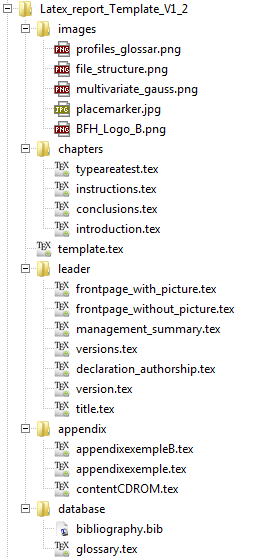
\includegraphics[scale=0.85]{images/file_structure.png}
%	\caption{File structure}
%	\label{fig:file_structure}
%\end{figure}

\section{Contact}
\label{sec:introduction_contact}

The manufacturers of this template welcome any suggestions for improvement. Chapter \ref{sec:introduction_suggestions} shows possible suggestions for improvement\index{suggestions}.

\begin{table}[H]
	\centering
		\begin{tabular}{lll} \toprule
			\textbf{First Name Last Name} & \textbf{E-mail} & \textbf{Function} \\ \midrule
			Alfred Kaufmann & alfred.kaufmann@bfh.ch & Employer, Project Management, \\
			& & Supplements, Improvements \\ \midrule
			Fritz Dellsperger & Retired & Tips on the structure and layout \\ \midrule
			David Burri & Contracted out & First compilation of the Template \\ \bottomrule
		\end{tabular}
	\caption{Contact Persons}
	\label{tab:Contact Persons}
\end{table}


\section{Suggestions for Improvement}
\label{sec:introduction_suggestions}

\begin{itemize}
	\item Create a BFH Style Files
	\item Template for the Compilation of presentations with \LaTeX{}
\end{itemize}


